%
% beispiel2.tex -- example of a non-tight frame in 2 dimensions
%
% (c) 2019 Prof Dr Andreas Müller, Hochschule Rapperswil
%
\documentclass[tikz]{standalone}
\usepackage{amsmath}
\usepackage{times}
\usepackage{txfonts}
\usepackage{pgfplots}
\usepackage{csvsimple}
\usetikzlibrary{arrows,intersections,math}
\begin{document}
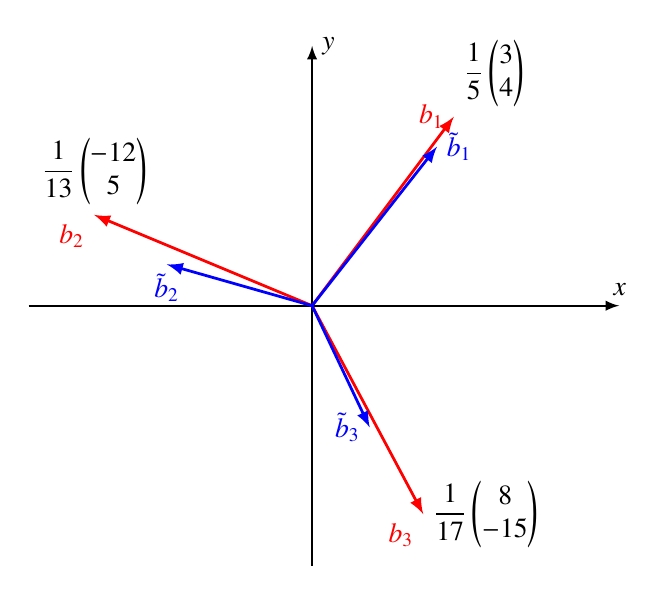
\begin{tikzpicture}[>=latex,scale=3]

\draw[->,line width=0.7pt] (-1.2,0)--(1.3,0) coordinate[label={$x$}];
\draw[->,line width=0.7pt] (0,-1.1)--(0,1.1) coordinate[label={right:$y$}];

\coordinate (B1) at ({3/5},{4/5});
\coordinate (B2) at ({-12/13},{5/13});
\coordinate (B3) at ({8/17},{-15/17});

\coordinate (C1) at ({4.259/8.053},{5.422/8.053});
\coordinate (C2) at ({-71.8432/116.7685},{40.8473/233.5370});
\coordinate (C3) at ({28.4716/116.7685},{-120.3549/233.5370});

\draw[->,line width=1pt,color=red] (0,0)--(B1);
\draw[->,line width=1pt,color=red] (0,0)--(B2);
\draw[->,line width=1pt,color=red] (0,0)--(B3);

\node at (B1) [above right]
	{$\displaystyle\frac15\begin{pmatrix}3\\4\end{pmatrix}$};

\node at (B2) [above]
	{$\displaystyle\frac1{13}\begin{pmatrix}-12\\5\end{pmatrix}$};
	
\node at (B3) [right]
	{$\displaystyle\frac1{17}\begin{pmatrix}8\\-15\end{pmatrix}$};

\draw[->,line width=1pt,color=blue] (0,0)--(C1);
\draw[->,line width=1pt,color=blue] (0,0)--(C2);
\draw[->,line width=1pt,color=blue] (0,0)--(C3);

\node[color=red] at (B1) [left] {$b_1$};
\node[color=red] at (B2) [below left] {$b_2$};
\node[color=red] at (B3) [below left] {$b_3$};

\node[color=blue] at (C1) [right] {$\tilde{b}_1$};
\node[color=blue] at (C2) [below] {$\tilde{b}_2$};
\node[color=blue] at (C3) [left] {$\tilde{b}_3$};

\end{tikzpicture}
\end{document}

